%*----------- SLIDE -------------------------------------------------------------
\begin{frame}[c]{Metodologia}
    %\transboxin[duration=1,direction=30]
    \begin{figure}
        \centering
        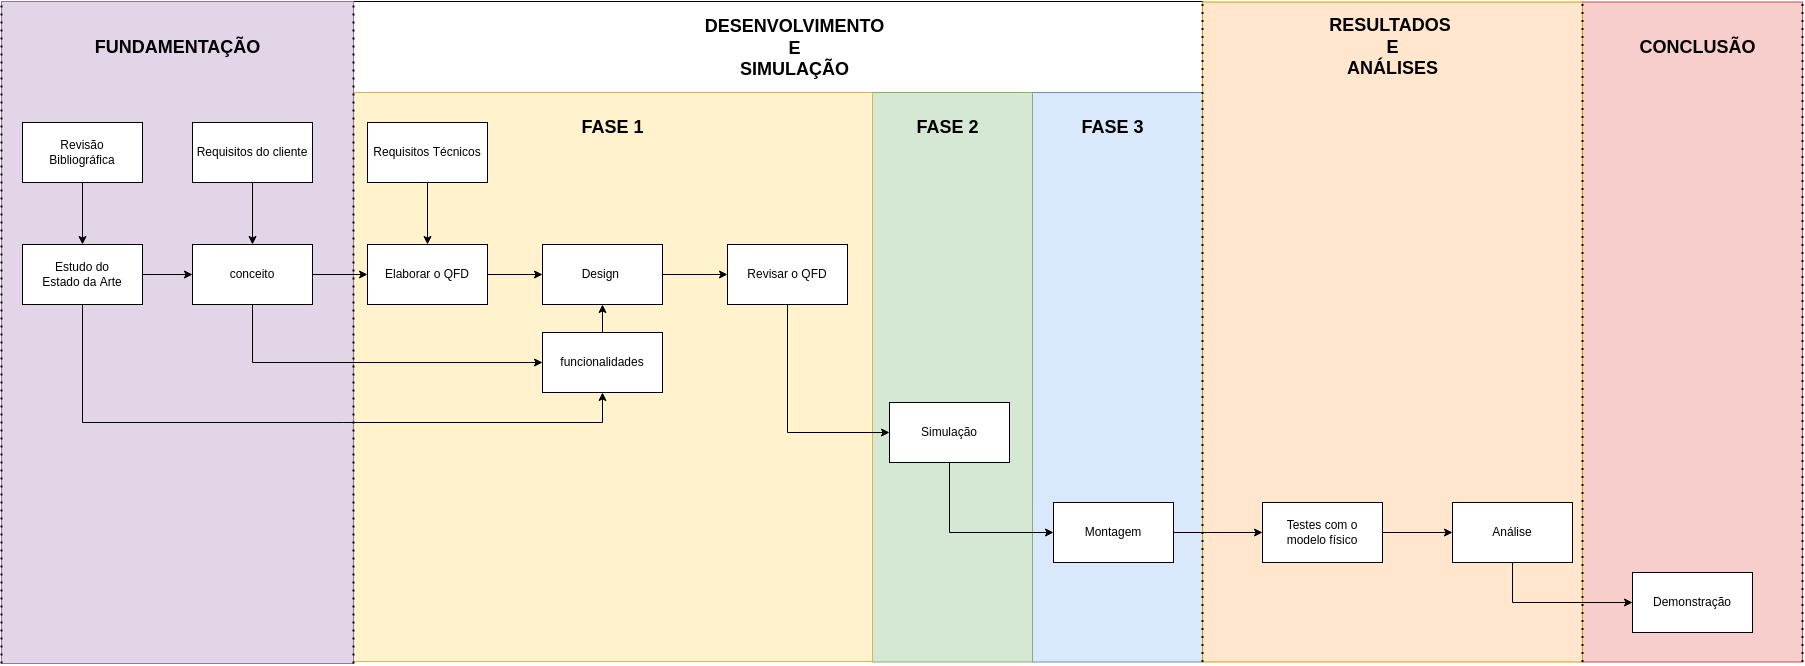
\includegraphics[width=1\textwidth]{metodologia.png}
    \end{figure}

%*----------- notes
    \note[item]{Notes can help you to remember important information. Turn on the notes option.}
\end{frame}
%-

% %*----------- SLIDE -------------------------------------------------------------
% \begin{frame}[c]{Roadmap}
%     %\cutpic{0.30cm}{3cm}{element}
%     \begin{tabular}{cccc}
%         \rule{30pt}{0ex}  &   \href{https://element.io/}{
\includegraphics[width=.2\textwidth]{element-1.png}} & \rule{15pt}{0ex} 
\includegraphics[width=.15\textwidth]{notion.png} \rule{15pt}{0ex}& 
\includegraphics[width=.16\textwidth]{github.png}\\
%     \end{tabular}

%     \begin{tabular}{ccc}
%         \phantom{This text s invisible} &   
\includegraphics[width=.2\textwidth]{trello.png} \rule{5pt}{0ex}& 
\includegraphics[width=.2\textwidth]{project-libre.png} \\
%     \end{tabular}
% %*----------- notes
%     \note[item]{Notes can help you to remember important information. Turn on the notes option.}
% \end{frame}
% %-